\scanpage{33}\mspage{32.}
% R2 independent reading, scan033 only. Every text line was read from the images.
% The arrow-like extension beside the initial cancelled glyph is kept as a drawing:
% its independence from that glyph, and its function, are not secure.
\deleted{\unsure{R|P}}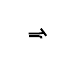
\begin{tikzpicture}[x=1ex,y=1ex,baseline=-.15ex]
\draw[line width=.65pt] (0,.15)--(.9,.15)--(1.35,.20);
\draw[line width=.65pt] (.05,-.08)--(.85,-.08)..controls(1.08,-.08)and(1.1,-.18)..(1.08,-.27);
\draw[line width=.7pt] (1.03,.55)--(1.48,-.05);
\end{tikzpicture}
1°) $\unsure{F|\mathcal F}\setminus G\subset F'\setminus G'$ i.e. Tout $A\in F\setminus G$ est $\notin G'$. En effet, si on avait $A\in G'$, on aurait $|A|\subset|G'|=|G|$ donc \deleted{$A\in$} (comme $G\leq F$) $A\in G$.

% Left note runs bottom-to-top. The long adjacent rule separates it from the body;
% the rule is not treated as a cancellation of the note.
\margin{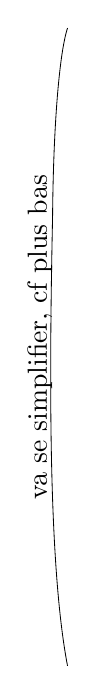
\begin{tikzpicture}[x=1cm,y=1cm,baseline=(m.south)]
\node[rotate=90,anchor=west,inner sep=0pt] (m) at (0,0) {va se simplifier, cf plus bas};
\draw[line width=.3pt] (.35,-2.1)..controls(.10,-.8)and(.12,1.7)..(.16,3.6)..controls(.17,4.8)and(.25,5.7)..(.35,6.0);
\end{tikzpicture}}

% 2°), four lines; two small cancelled superscripts survive in the bracketed group.
2°) $F'\setminus G'\subset F\setminus G$ Soit $A'\in F'\setminus G'$, prouvons $A'\in F\setminus G$, et d'abord $A'\in F$. \deleted{On a} Soit $A$ le plus petit él. de $F^{A'}$ donc
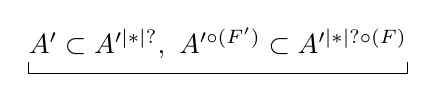
\begin{tikzpicture}[baseline=(s.base)]
\node[inner sep=0pt] (s) {$A'\subset A^{\deleted{\unsure{\prime|\ast|?}}},\ A'^{\circ(F')}\subset A^{\deleted{\unsure{\prime|\ast|?}}\circ(F)}$};
\draw[line width=.4pt] ([yshift=-1pt]s.south west)--([yshift=-5pt]s.south west)--([yshift=-5pt]s.south east)--([yshift=-1pt]s.south east);
\end{tikzpicture}
% Focused recheck: the two heavy final bars read =. A thinner curved tip,
% left connection and short inner bar are retained as an overwritten earlier
% relation, preferably element-of; its exact form/layer remains uncertain.
prouvons que $A'\deleted{\unsure{\in|\subset}}=A$ (d'où $A\in F$). \deleted{On a}

% Focused supplement: pale remnants beside Je dis; no word, mathematical sign,
% or deletion/insertion function is assigned to these marks.
\llap{\begin{tikzpicture}[x=1cm,y=1cm,baseline=0cm]
\draw[black!40,line width=.35pt] (.42,.44)--(.66,.64);
\draw[black!24,line width=.3pt] (.40,.31)..controls(.49,.25)and(.47,.21)..(.44,.16);
\draw[black!20,line width=.35pt,dash pattern=on 2pt off 1pt] (-.22,-.43)--(.12,-.24);
\draw[black!31,line width=.4pt] (.13,-.24)--(.28,-.17);
\end{tikzpicture}\hspace{.35em}}
Je dis que $A\in F\setminus G$ i.e. $A\notin G$, sinon on aurait $A\subset|G|=|G'|$ donc $A'\in G'$ puisque $A'\in F'$ et $G'\leq F'$, absurde. \deleted{Mais} Donc $A\in F\setminus G$, donc $A\in F'$, \deleted{et} Il en résulte que $A^{\circ(F)}=A^{\circ(F')}$ (car $F'\preceq F$\inserted{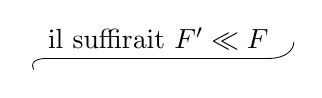
\begin{tikzpicture}[baseline=(n.base)]
\node[inner sep=0pt,anchor=west] (n) {il suffirait $F'\ll F$};
\draw[line width=.3pt] ([xshift=-5pt,yshift=-7pt]n.south west)..controls([xshift=-7pt,yshift=-3pt]n.south west)and([xshift=-1pt,yshift=-3pt]n.south west)..([yshift=-3pt]n.south west)--([yshift=-3pt]n.south east)..controls([xshift=6pt,yshift=-3pt]n.south east)and([xshift=9pt,yshift=0pt]n.south east)..([xshift=9pt,yshift=3pt]n.south east);
\end{tikzpicture}}\deleted{)} cf lemme plus bas) et \deleted{\unsure{bien}} \deleted{$\unsure{F|\in}$} $A,A'\in F'$ tels que $A'^{\circ(F')}\subset A^{\circ(F')}$, ce qui prouve $A=A'$.

Donc \unsure{on a} prouvé que $\deleted{\unsure{F|A}}A'\in F'\setminus G'\Rightarrow A'\in F$. Prouvons qu'on a $A'\notin G$ (d'où $A'\in F\setminus G$\deleted{)}, qed). Sinon on aurait $A'\in G$, on aurait $A'\subset |G|=|G'|$, d'où (comme $A'\in F'$
% A pale left-pointing arrow-like trace lies above et. Possibly erased; neither
% its status nor its target is secure. It is reproduced without assigning a word.
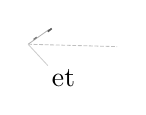
\begin{tikzpicture}[baseline=(e.base),x=1cm,y=1cm]
\node[inner sep=0pt] (e) at (0,0) {et};
\draw[black!25,line width=.3pt,dash pattern=on 1.4pt off .6pt] (-.45,.43)--(.68,.40);
\draw[black!30,line width=.3pt] (-.45,.43)--(-.18,.62);
\draw[black!20,line width=.3pt] (-.45,.43)--(-.20,.16);
\draw[black!65,line width=.6pt] (-.20,.59)--(-.15,.63);
\draw[black!50,line width=.5pt] (-.38,.49)--(-.34,.52);
\end{tikzpicture}
$G'\leq F'$) $A'\in G'$, absurde.

% First draft of b) => c), diagonally hatched. The last Prouvons line lies below
% the actual ends of the hatch strokes: its cancellation is inferred from the
% draft's block association, not from a stroke through that line.
% The curved stroke under On suppose is an insertion leader, not a literal (.
% The underline ends before F'. The a of strate is extremely reduced/dot-like.
\deleted{b) $\Rightarrow$ c) \inserted{\begin{tikzpicture}[baseline=(n.base)]
\node[inner sep=0pt,anchor=west] (n) {On suppose b) i.e. $\varphi$ induit $F'\setminus G'\overset{\sim}{\longrightarrow}F\setminus G$};
\draw[line width=.3pt] ([xshift=-6pt,yshift=-10pt]n.south west)..controls([xshift=-10pt,yshift=-2pt]n.south west)and([xshift=1pt,yshift=-3pt]n.south west)..([xshift=6pt,yshift=-3pt]n.south west)--([yshift=-3pt]n.south east)..controls([xshift=6pt,yshift=-3pt]n.south east)and([xshift=9pt,yshift=-1pt]n.south east)..([xshift=9pt,yshift=3pt]n.south east);
\end{tikzpicture}} Soit $A\in F\setminus G$, prouvons que $A^{\circ(F)}$ est une \uline{strate ouverte \deleted{dans \unsure{la}} de} $F'$. Soit $A'\in F'\setminus G'$ l'unique élément \deleted{de} tel que $\varphi(A')=A$. Prouvons $A'^{\circ(F')}=A^{\circ(F)}$.}

b $\Longleftrightarrow$ c \deleted{Posons} On a $|F|\setminus|G|=|F'|\setminus|G'|$, soit $U$, Posons $F\setminus G=I^{\unsure{\ast|k|+}},\ F'\deleted{\unsure{\times|\setminus}}\unsure{\setminus}G'=I'^{\unsure{\ast|k|+}}$ (parties ouvertes des ens d'indices ordonnés $I$, \deleted{$\unsure{A|\Delta}$} $(=F)$, $I'(=F')$. On a
% The outer ( before parties has no visible closing partner on this page.
